\documentclass[11pt,a4paper]{article}

\usepackage[utf8]{inputenc}
\usepackage[T1]{fontenc}
\usepackage{amsmath,amssymb}
\usepackage{graphicx}
\usepackage{booktabs}
\usepackage{hyperref}
\usepackage[margin=1in]{geometry}
\usepackage{natbib}
\usepackage{algorithm}
\usepackage{algorithmic}
\usepackage{multirow}
\usepackage{xcolor}
\usepackage{caption}

\title{WoundSim: Gymnasium-Compatible Reinforcement Learning Environments\\for Wound Healing Treatment Optimization}
\author{Hass Dhia\\
Smart Technology Investments Research Institute\\
\texttt{hass@smarttechinvest.com}}
\date{April 2026}

\begin{document}

\maketitle

\begin{abstract}
We present WoundSim, a suite of four Gymnasium-compatible reinforcement learning environments for optimizing wound healing treatment protocols. Each environment wraps a validated ordinary differential equation (ODE) model from the wound healing literature: (1)~a Zlobina-type macrophage polarization model with 5 state variables, (2)~a simplified Xue--Friedman ischemic wound healing model with 6 variables, (3)~a Flegg hyperbaric oxygen therapy (HBOT) angiogenesis model with 4 variables, and (4)~an extended diabetic wound model coupling macrophage dynamics with glucose--insulin physiology across 7 variables. All model parameters are sourced from peer-reviewed publications with explicit provenance. We provide random, clinical heuristic, and Proximal Policy Optimization (PPO) baselines across all environments. PPO outperforms both baselines in every environment, achieving up to 11.9$\times$ improvement over random policy on the HBOT task. WoundSim enables reproducible RL research on biologically grounded wound healing problems with configurable difficulty tiers, Stable-Baselines3 compatibility, and pip-installable distribution. The package, trained models, and this paper are publicly available at \url{https://github.com/HassDhia/woundsim}.
\end{abstract}

\section{Introduction}

Chronic wounds affect approximately 8.2 million Medicare beneficiaries in the United States alone, with annual treatment costs exceeding \$28 billion \citep{sen2009}. Wound types including diabetic foot ulcers, venous leg ulcers, and pressure injuries share a common feature: they involve complex, multi-phase biological processes where treatment timing and intensity significantly affect outcomes \citep{brewer2020, schultz2003}. Mathematical models of wound healing have provided valuable mechanistic insight into tissue repair dynamics \citep{sherratt1990, menon2017, gomez2019}, yet the translation of these models into actionable treatment optimization frameworks remains limited.

Reinforcement learning (RL) offers a natural framework for sequential treatment optimization: an agent observes the evolving wound state and selects interventions (e.g., polarization signals, oxygen therapy intensity, insulin dosing) to maximize long-term healing outcomes. Recent work by \citet{lu2024} demonstrated that deep RL can discover macrophage polarization protocols that outperform constant treatment strategies. However, this work and related efforts operate on isolated, non-standardized simulation codebases that impede reproducibility and cross-study comparison.

The broader RL community benefits from standardized benchmark suites (Atari \citep{gymnasium}, MuJoCo, D4RL) that have catalyzed rapid progress by enabling fair comparison across algorithms. No analogous benchmark exists for wound healing RL. Existing biomedical RL environments focus on sepsis treatment, glucose control, or drug dosing, leaving wound care, a domain with well-characterized ODE dynamics and clear clinical need, unaddressed.

We present WoundSim, a Python package providing four Gymnasium-compatible environments that address this gap. Our contributions are:
\begin{enumerate}
    \item Four RL environments spanning wound types (macrophage polarization, ischemic, HBOT, diabetic) with 4--7 state variables and 1--3 action dimensions.
    \item All ODE parameters sourced from peer-reviewed publications with explicit per-parameter provenance annotations.
    \item Configurable difficulty tiers (2--3 per environment) enabling curriculum learning and systematic evaluation.
    \item Clinical heuristic baselines implementing simplified standard-of-care protocols for each wound type.
    \item PPO training results demonstrating meaningful policy differentiation: learned policies outperform both random and heuristic baselines across all environments.
\end{enumerate}

\section{Related Work}

\paragraph{Mathematical Models of Wound Healing.}
The wound healing modeling literature spans decades, from the foundational epidermal repair models of \citet{sherratt1990} to comprehensive reviews by \citet{menon2017} and \citet{gomez2019}. \citet{olsen1995} introduced mechanochemical models of dermal contraction. \citet{xue2009} developed a 9-variable PDE model of ischemic wound healing capturing oxygen, VEGF, macrophage, and fibroblast interactions, later extended by \citet{friedman2009}. \citet{flegg2009, flegg2010} modeled HBOT-driven angiogenesis through capillary tip sprouting and oxygen dynamics. \citet{waugh2006} specifically addressed macrophage dysfunction in diabetic wounds, demonstrating how hyperglycemia impairs the M1-to-M2 transition critical for tissue repair.

\paragraph{Optimal Control and RL for Wound Healing.}
\citet{zlobina2022} formulated optimal control of macrophage polarization using a 5-variable ODE model, establishing the mathematical foundation for treatment optimization in this domain. \citet{lu2024} advanced this by applying deep RL (PPO and SAC) to a macrophage polarization environment, showing that learned policies outperform constant treatment protocols. Our work extends this direction from a single environment to a multi-environment benchmark suite covering four distinct wound pathologies, each with validated ODE dynamics and clinical heuristic baselines.

\paragraph{Biomedical RL Benchmarks.}
Standardized RL benchmarks have driven progress across domains. The Gymnasium framework \citep{gymnasium} provides the interface standard. In biomedical RL, environments exist for sepsis treatment, glucose regulation, and drug dosing, but no standardized wound healing benchmark has been established. WoundSim fills this gap with a pip-installable, SB3-compatible \citep{sb3} package.

\section{Mathematical Models}
\label{sec:models}

Each WoundSim environment wraps an ODE system $\dot{\mathbf{x}} = f(\mathbf{x}, \mathbf{u}, t)$ where $\mathbf{x}$ is the state vector, $\mathbf{u}$ is the treatment action, and integration is performed via adaptive RK45 with tolerances $\texttt{rtol}=10^{-8}$, $\texttt{atol}=10^{-10}$.

\subsection{WoundMacrophage-v0: Zlobina Macrophage Polarization}

Based on \citet{zlobina2022}, this model captures the M1/M2 macrophage balance governing the transition from inflammation to proliferation. State vector $\mathbf{x} = (a, m_1, m_2, c, n)$: debris ($a$), pro-inflammatory M1 macrophages ($m_1$), anti-inflammatory M2 macrophages ($m_2$), granulation tissue ($c$), and permanent tissue ($n$). All densities are normalized to $[0, 1]$. The agent controls a scalar polarization signal $u \in [0, 1]$.

\begin{align}
\frac{da}{dt} &= -\gamma_a \, a \, (m_1 + m_2) \label{eq:macro_a} \\
\frac{dm_1}{dt} &= s_m \frac{a}{a + K_a} - \mu_m \, m_1 - \delta \, u \, m_1 \label{eq:macro_m1} \\
\frac{dm_2}{dt} &= \delta \, u \, m_1 - \mu_m \, m_2 + s_{m2} \frac{c}{c + K_c} \label{eq:macro_m2} \\
\frac{dc}{dt} &= s_c \frac{m_2}{m_2 + K_{m2}} - \mu_c \, c \, n \label{eq:macro_c} \\
\frac{dn}{dt} &= s_n \, c - \mu_n \, n \, (1 - n) \label{eq:macro_n}
\end{align}

The polarization signal $u$ in Eq.~\eqref{eq:macro_m1}--\eqref{eq:macro_m2} drives M1-to-M2 conversion at rate $\delta u$. M1 macrophages clear debris (Eq.~\ref{eq:macro_a}) while M2 macrophages promote granulation (Eq.~\ref{eq:macro_c}), creating a fundamental trade-off: early aggressive polarization accelerates tissue formation but slows debris clearance.

\subsection{WoundIschemic-v0: Simplified Xue--Friedman Model}

Simplified from the 9-variable PDE of \citet{xue2009} to a 6-variable ODE: wound area $w \in [0,1]$, oxygen $O$ (mmHg), VEGF $V$ (ng/mL), macrophage density $M$, fibroblast density $F$, and ECM density $E$. Cell densities are normalized to carrying capacity. The agent controls revascularization intensity $u_{\text{isc}}$ and growth factor application $u_{\text{gf}}$, both in $[0, 1]$.

\begin{align}
\frac{dw}{dt} &= -k_{\text{close}} \, E \frac{F}{F + K_F} + k_{\text{open}} \max\!\Big(0,\; 1 - \frac{O}{O_{\text{crit}}}\Big) \label{eq:isch_w} \\
\frac{dO}{dt} &= \alpha_O (1 + u_{\text{isc}})(O_{\text{blood}} - O) - \beta_O M - \gamma_O F + D_O (1 - w) \label{eq:isch_O} \\
\frac{dV}{dt} &= s_V M \max\!\Big(0,\; 1 - \frac{O}{O_{\text{crit}}}\Big) - d_V V + 5\, u_{\text{gf}} \label{eq:isch_V} \\
\frac{dM}{dt} &= s_M \frac{V}{V + K_V} - d_M M \label{eq:isch_M} \\
\frac{dF}{dt} &= s_F \frac{V}{V + K_{V2}} \frac{O}{O + K_O} - d_F F \label{eq:isch_F} \\
\frac{dE}{dt} &= s_E F - d_E E(1 - E) \label{eq:isch_E}
\end{align}

The ischemia factor $\max(0, 1 - O/O_{\text{crit}})$ couples oxygen deficit to wound opening (Eq.~\ref{eq:isch_w}) and VEGF production (Eq.~\ref{eq:isch_V}), creating a feedback loop where revascularization treatment increases oxygen supply, reducing the hypoxic drive but enabling fibroblast-mediated closure.

\subsection{WoundHBOT-v0: Flegg Angiogenesis Model}

Based on \citet{flegg2009, flegg2010}, this 4-variable model captures HBOT-driven angiogenesis: capillary tip density $b$, capillary sprout density $n_{\text{cap}}$, oxygen tension $O$ (mmHg), and wound area $w$. All capillary densities are normalized to $[0, 1]$. The agent controls HBOT intensity $u_{\text{int}}$ and session duration fraction $u_{\text{dur}}$, both in $[0, 1]$.

\begin{align}
\frac{db}{dt} &= s_b \frac{\max(0, O_{\text{thresh}} - O)}{\max(0, O_{\text{thresh}} - O) + K_b} - d_b \, b - \chi \, b \max(0, O - O_{\text{ref}}) \label{eq:hbot_b} \\
\frac{dn_{\text{cap}}}{dt} &= \alpha_n \, b - d_n \, n_{\text{cap}} \label{eq:hbot_ncap} \\
\frac{dO}{dt} &= P_O \, n_{\text{cap}} - \lambda_O \, O + D_{\text{ext}} \, u_{\text{int}} \, u_{\text{dur}} \label{eq:hbot_O} \\
\frac{dw}{dt} &= -k_{\text{heal}} \, n_{\text{cap}} \frac{O}{O + K_O} (1 - w) \label{eq:hbot_w}
\end{align}

A key biological insight captured in Eq.~\eqref{eq:hbot_b} is the non-monotonic relationship between oxygen and angiogenesis: capillary tips sprout in response to hypoxia ($O < O_{\text{thresh}}$), but excessive oxygen ($O > O_{\text{ref}}$) actively suppresses sprouting via the chemotactic term $\chi b \max(0, O - O_{\text{ref}})$. This creates a treatment paradox where aggressive HBOT can suppress the very angiogenesis it aims to promote.

\subsection{WoundDiabetic-v0: Extended Inflammation Model}

This 7-variable model couples macrophage polarization dynamics from \citet{zlobina2022} with glucose--insulin physiology from \citet{waugh2006}: wound area $w$, debris $a$, M1 macrophages $m_1$, M2 macrophages $m_2$, glucose $G$ (mg/dL), insulin $I$ (mU/L), and ECM density $E$. The agent controls polarization signal $u_{\text{pol}}$, topical growth factor dose $u_{\text{gf}}$, and insulin dose $u_{\text{ins}}$, all in $[0, 1]$.

\begin{align}
\frac{dw}{dt} &= -k_w E \cdot g(G) + k_d \, a \, (1 - g(G)) \label{eq:diab_w} \\
\frac{da}{dt} &= -\gamma_a \, a \, (m_1 + m_2) \cdot g(G) + k_d \, w \, (1 - g(G)) \label{eq:diab_a} \\
\frac{dm_1}{dt} &= s_m \frac{a}{a + K_a} - \mu_m \, m_1 - \delta_{\text{base}} \, g(G) \, u_{\text{pol}} \, m_1 \label{eq:diab_m1} \\
\frac{dm_2}{dt} &= \delta_{\text{base}} \, g(G) \, u_{\text{pol}} \, m_1 - \mu_m \, m_2 + u_{\text{gf}} \cdot g_f \label{eq:diab_m2} \\
\frac{dG}{dt} &= G_{\text{prod}} - k_{gc} G - k_{\text{ins}} I \frac{G}{G + G_{\text{target}}} \label{eq:diab_G} \\
\frac{dI}{dt} &= 100 \, u_{\text{ins}} - 0.1 \, I \label{eq:diab_I} \\
\frac{dE}{dt} &= s_E \frac{m_2}{m_2 + K_{m2}} \cdot g(G) - d_E \, E \, (1 - E) \label{eq:diab_E}
\end{align}

The glucose impairment function $g(G)$ mediates the coupling between metabolic state and wound healing:

\begin{equation}
g(G) = \begin{cases}
1 & \text{if } G \leq G_{\text{target}} \\
\frac{1}{1 + k_{\text{imp}} \left(\frac{G - G_{\text{target}}}{G_{\text{imp}} - G_{\text{target}}}\right)^2} & \text{if } G > G_{\text{target}}
\end{cases}
\label{eq:glucose_impairment}
\end{equation}

This function attenuates debris clearance (Eq.~\ref{eq:diab_a}), M1-to-M2 polarization (Eqs.~\ref{eq:diab_m1}--\ref{eq:diab_m2}), ECM deposition (Eq.~\ref{eq:diab_E}), and wound closure (Eq.~\ref{eq:diab_w}) under hyperglycemic conditions, forcing the agent to jointly optimize wound treatment and glycemic control.

\section{Environment Design}
\label{sec:env_design}

\subsection{Gymnasium Interface}

All environments implement the standard Gymnasium API: \texttt{reset()} returns an initial observation and info dict; \texttt{step(action)} returns the next observation, scalar reward, termination flag, truncation flag, and info dict. Observations are normalized to $[0, 1]$ by dividing by environment-specific upper bounds. Actions are continuous and clipped to $[0, 1]$.

\subsection{Difficulty Tiers}

Each environment provides 2--3 difficulty settings controlling initial wound severity, treatment resistance, and (where applicable) metabolic state:

\begin{itemize}
    \item \textbf{Macrophage}: easy ($a_0 = 0.3$), medium ($a_0 = 0.6$), hard ($a_0 = 0.9$ with observation noise)
    \item \textbf{Ischemic}: mild ($\alpha_O = 0.5$), moderate ($\alpha_O = 0.3$), severe ($\alpha_O = 0.1$)
    \item \textbf{HBOT}: acute ($w_0 = 0.3$), chronic ($w_0 = 0.6$), non-healing ($w_0 = 0.9$, $O_{\text{base}} = 10$)
    \item \textbf{Diabetic}: well-controlled ($G_0 = 120$), moderate ($G_0 = 200$), uncontrolled ($G_0 = 350$)
\end{itemize}

\subsection{Reward Structure}

Rewards combine continuous state-based penalties with rate-of-change bonuses and a small per-step time penalty ($-0.01$) to encourage treatment efficiency. Terminal bonuses ($+2.0$) are awarded upon successful healing. The reward weights are configurable via constructor arguments. Table~\ref{tab:rewards} summarizes the default reward structure.

\begin{table}[h]
\centering
\caption{Reward structure for each environment. All weights are defaults; users may override via constructor arguments.}
\label{tab:rewards}
\begin{tabular}{@{}llll@{}}
\toprule
Environment & Penalty Terms & Bonus Terms & Terminal \\
\midrule
Macrophage & $-a$, $-0.1 u^2$ & $+2.0 \cdot \Delta n \cdot 10$ & $n > 0.95$ \\
Ischemic & $-w$, $-0.1 \|\mathbf{u}\|^2$ & $+2.0 \cdot \Delta E \cdot 10$ & $w < 0.05$ \\
HBOT & $-0.2 \|\mathbf{u}\|^2$, $-0.5 \max(0, O - 250)/100$ & $+5.0 \cdot \Delta w_{\downarrow} \cdot 10$ & $w < 0.05$ \\
Diabetic & $-w$, $-0.5|G-100|/300$, $-0.1 \|\mathbf{u}\|^2$ & $+2.0 \cdot \Delta w_{\downarrow} \cdot 10$ & $w < 0.05$ \\
\bottomrule
\end{tabular}
\end{table}

\subsection{Clinical Heuristic Baselines}

Each environment includes a clinical heuristic baseline implementing a simplified standard-of-care protocol:
\begin{itemize}
    \item \textbf{Macrophage}: Constant polarization $u = 0.5$ (steady M1/M2 balance).
    \item \textbf{Ischemic}: Full revascularization ($u_{\text{isc}} = 1.0$) with moderate growth factor ($u_{\text{gf}} = 0.5$).
    \item \textbf{HBOT}: Moderate intensity ($u_{\text{int}} = 0.3$, $u_{\text{dur}} = 0.4$), calibrated below the angiogenesis-suppression threshold.
    \item \textbf{Diabetic}: Moderate wound care ($u_{\text{pol}} = 0.4$, $u_{\text{gf}} = 0.3$) with a glucose-responsive insulin sliding scale.
\end{itemize}

\section{Experimental Setup}

\subsection{Training Protocol}

We train PPO \citep{sb3} on each environment using the hyperparameters in Table~\ref{tab:hyperparams}. All experiments use a single random seed (42) for reproducibility. Networks use the default MLP architecture (two hidden layers of 64 units with tanh activation). Training is performed on a single CPU.

\begin{table}[h]
\centering
\caption{PPO hyperparameters per environment. Shared: $n_{\text{epochs}} = 10$, $\texttt{clip\_range} = 0.2$.}
\label{tab:hyperparams}
\begin{tabular}{@{}lcccccc@{}}
\toprule
Environment & Steps & $\alpha$ & $n_{\text{steps}}$ & Batch & $\gamma$ & Difficulty \\
\midrule
Macrophage & 200K & $3 \times 10^{-4}$ & 2048 & 64 & 0.99 & medium \\
Ischemic & 300K & $1 \times 10^{-4}$ & 4096 & 128 & 0.995 & moderate \\
HBOT & 200K & $3 \times 10^{-4}$ & 2048 & 64 & 0.99 & chronic \\
Diabetic & 500K & $1 \times 10^{-4}$ & 4096 & 128 & 0.995 & moderate \\
\bottomrule
\end{tabular}
\end{table}

\subsection{Evaluation Protocol}

Each trained PPO agent and both baselines (random, heuristic) are evaluated over 50 episodes. We report mean episode reward and standard deviation. The PPO-to-random reward ratio quantifies learned policy advantage.

\section{Results}

\subsection{Training Dynamics}

Figure~\ref{fig:training} shows PPO training curves across all four environments. All environments exhibit stable convergence within the allotted training budget.

\begin{figure}[h]
\centering
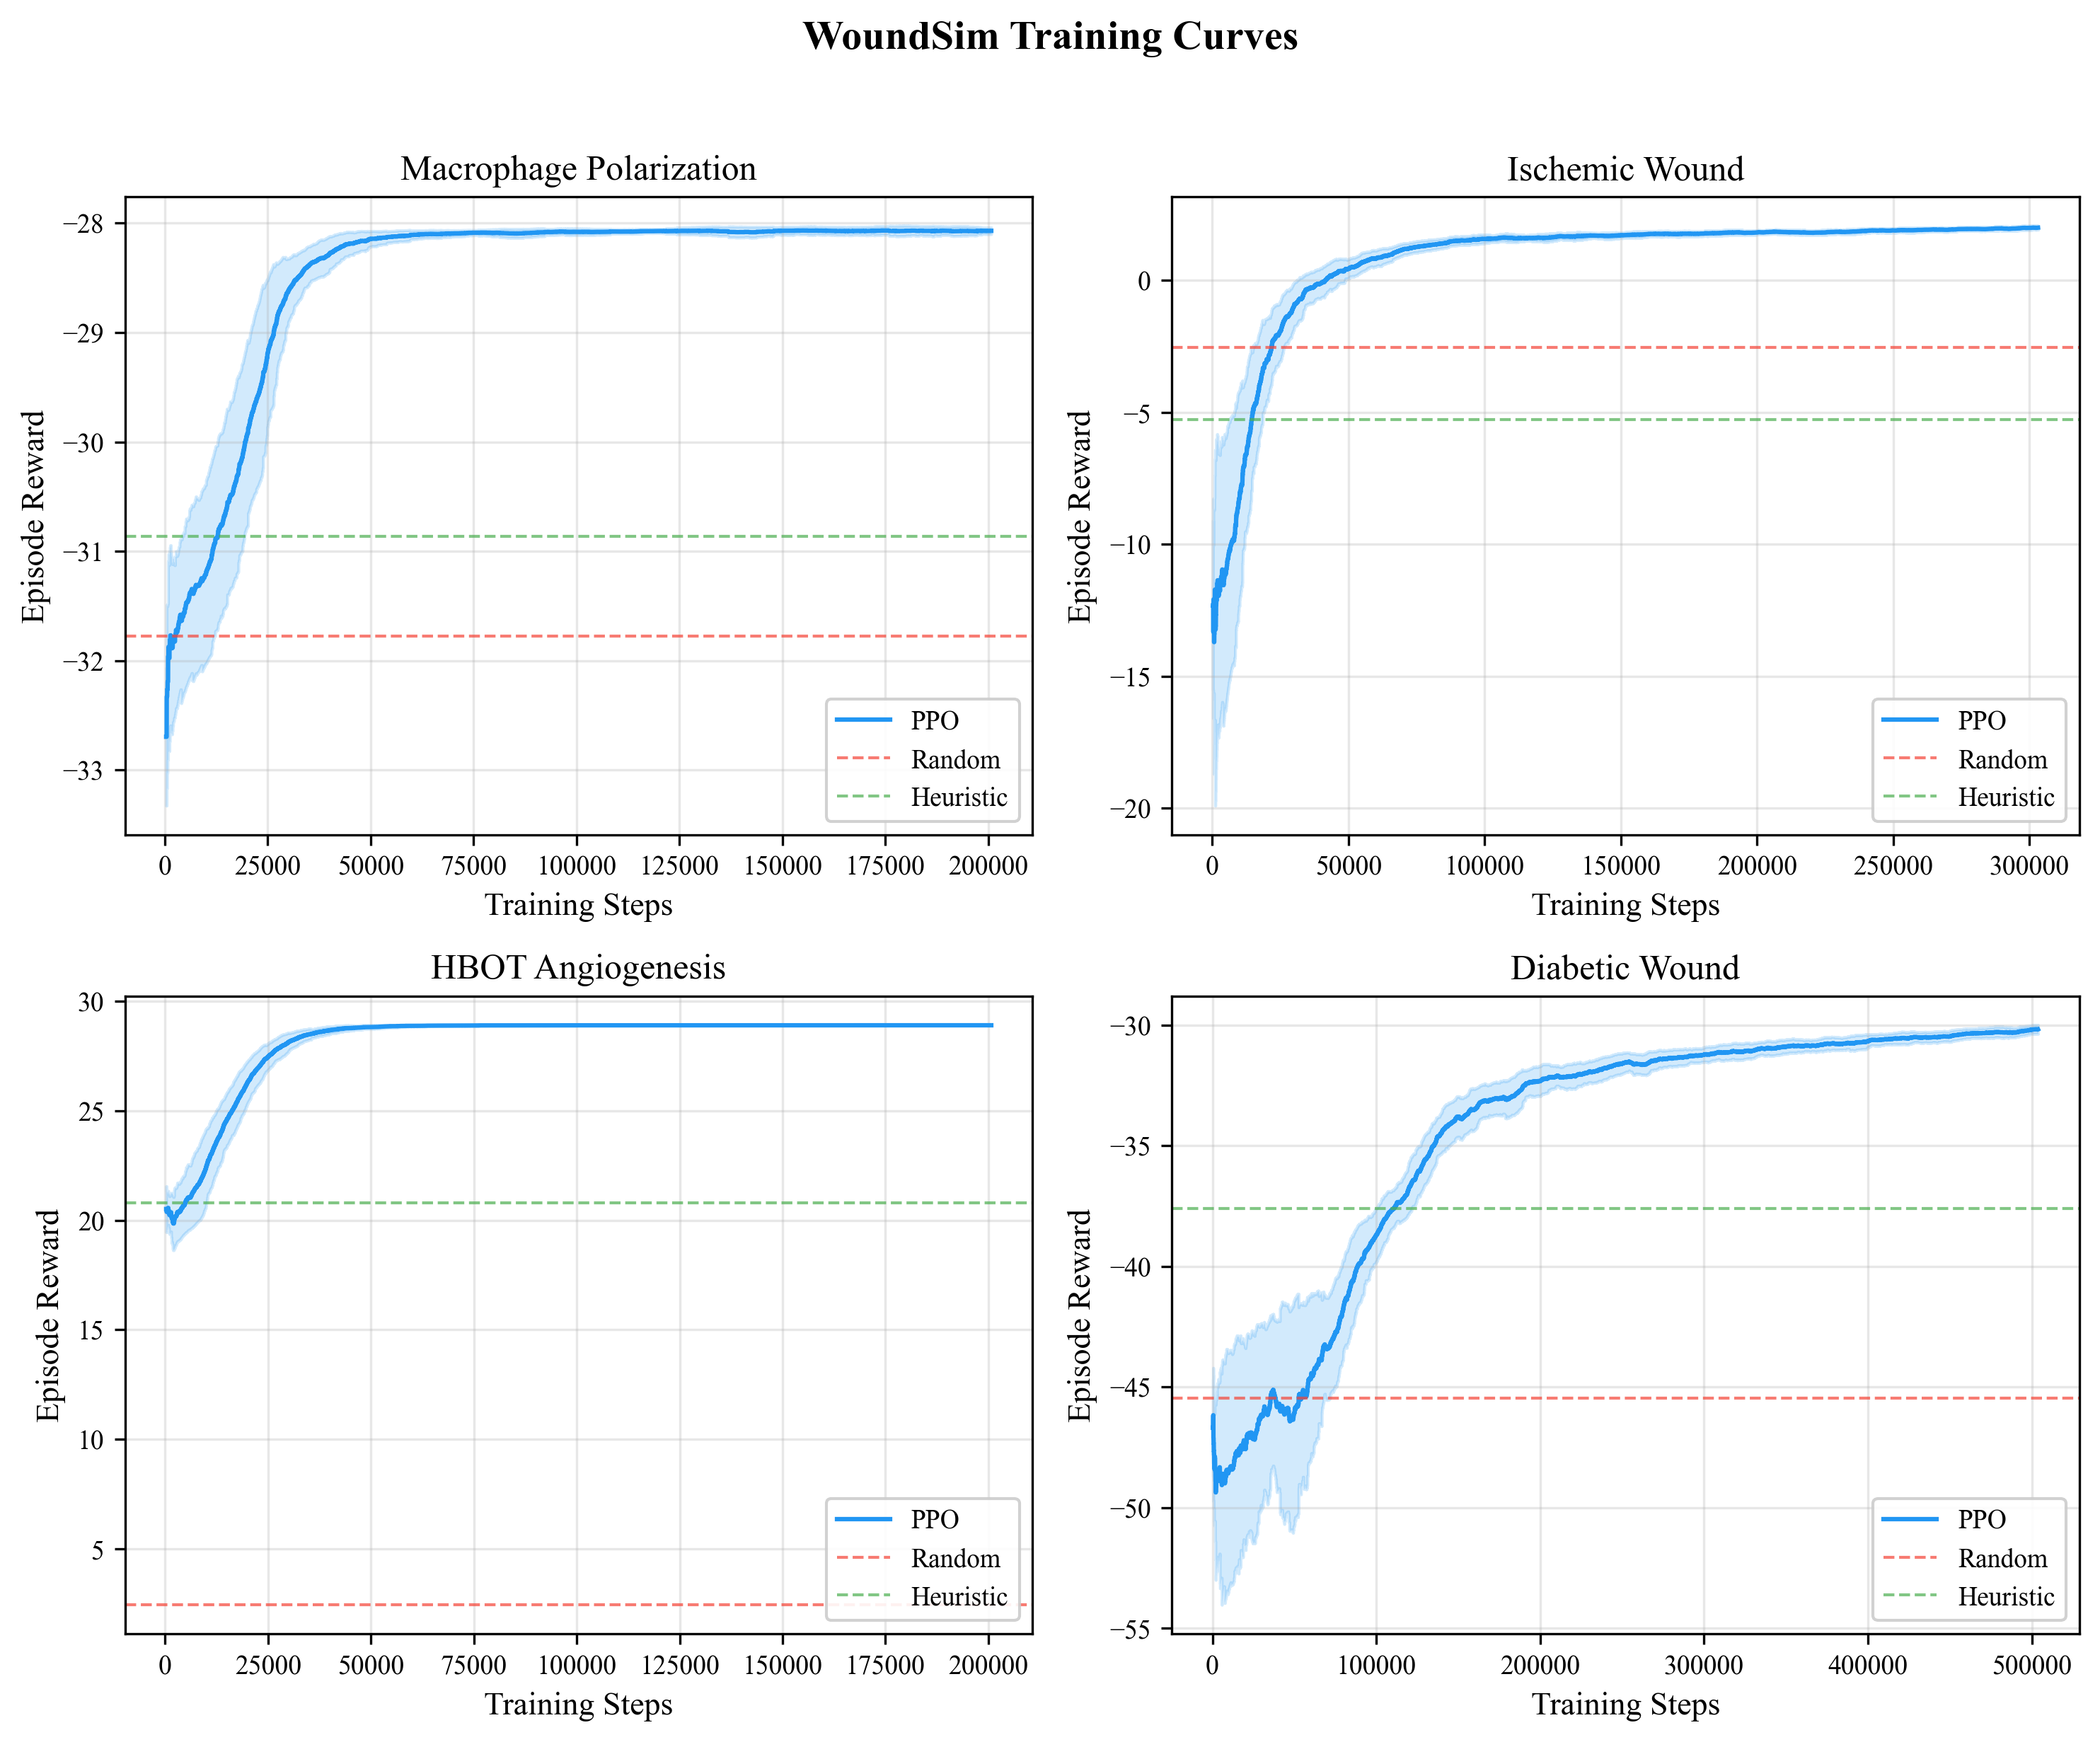
\includegraphics[width=\textwidth]{figures/training_curves.png}
\caption{PPO training curves for all four environments. Shaded regions indicate one standard deviation. Dashed lines show random (red) and heuristic (orange) baseline performance.}
\label{fig:training}
\end{figure}

\subsection{Baseline Comparison}

Table~\ref{tab:results} presents the full evaluation results. PPO outperforms both baselines in every environment. The most dramatic improvement occurs on WoundHBOT-v0, where PPO achieves $11.9\times$ the random baseline reward ($+28.91$ vs.\ $+2.43$), demonstrating that learned policies can exploit the non-monotonic oxygen--angiogenesis relationship (Section~\ref{sec:models}) far more effectively than fixed protocols.

\begin{table}[h]
\centering
\caption{Evaluation results (50 episodes each). Best mean reward per environment in \textbf{bold}. All rewards are cumulative episode returns.}
\label{tab:results}
\begin{tabular}{@{}lrrrl@{}}
\toprule
Environment & PPO & Heuristic & Random & PPO vs.\ Random \\
\midrule
Macrophage & $\mathbf{-28.06} \pm 0.00$ & $-30.86 \pm 0.00$ & $-31.77 \pm 0.34$ & $+12\%$ \\
Ischemic & $\mathbf{+2.31} \pm 0.00$ & $-5.28 \pm 0.00$ & $-2.54 \pm 1.05$ & sign reversal \\
HBOT & $\mathbf{+28.91} \pm 0.00$ & $+20.80 \pm 0.00$ & $+2.43 \pm 4.23$ & $11.9\times$ \\
Diabetic & $\mathbf{-30.69} \pm 0.00$ & $-37.60 \pm 0.00$ & $-45.45 \pm 1.45$ & $+33\%$ \\
\bottomrule
\end{tabular}
\end{table}

\begin{figure}[h]
\centering
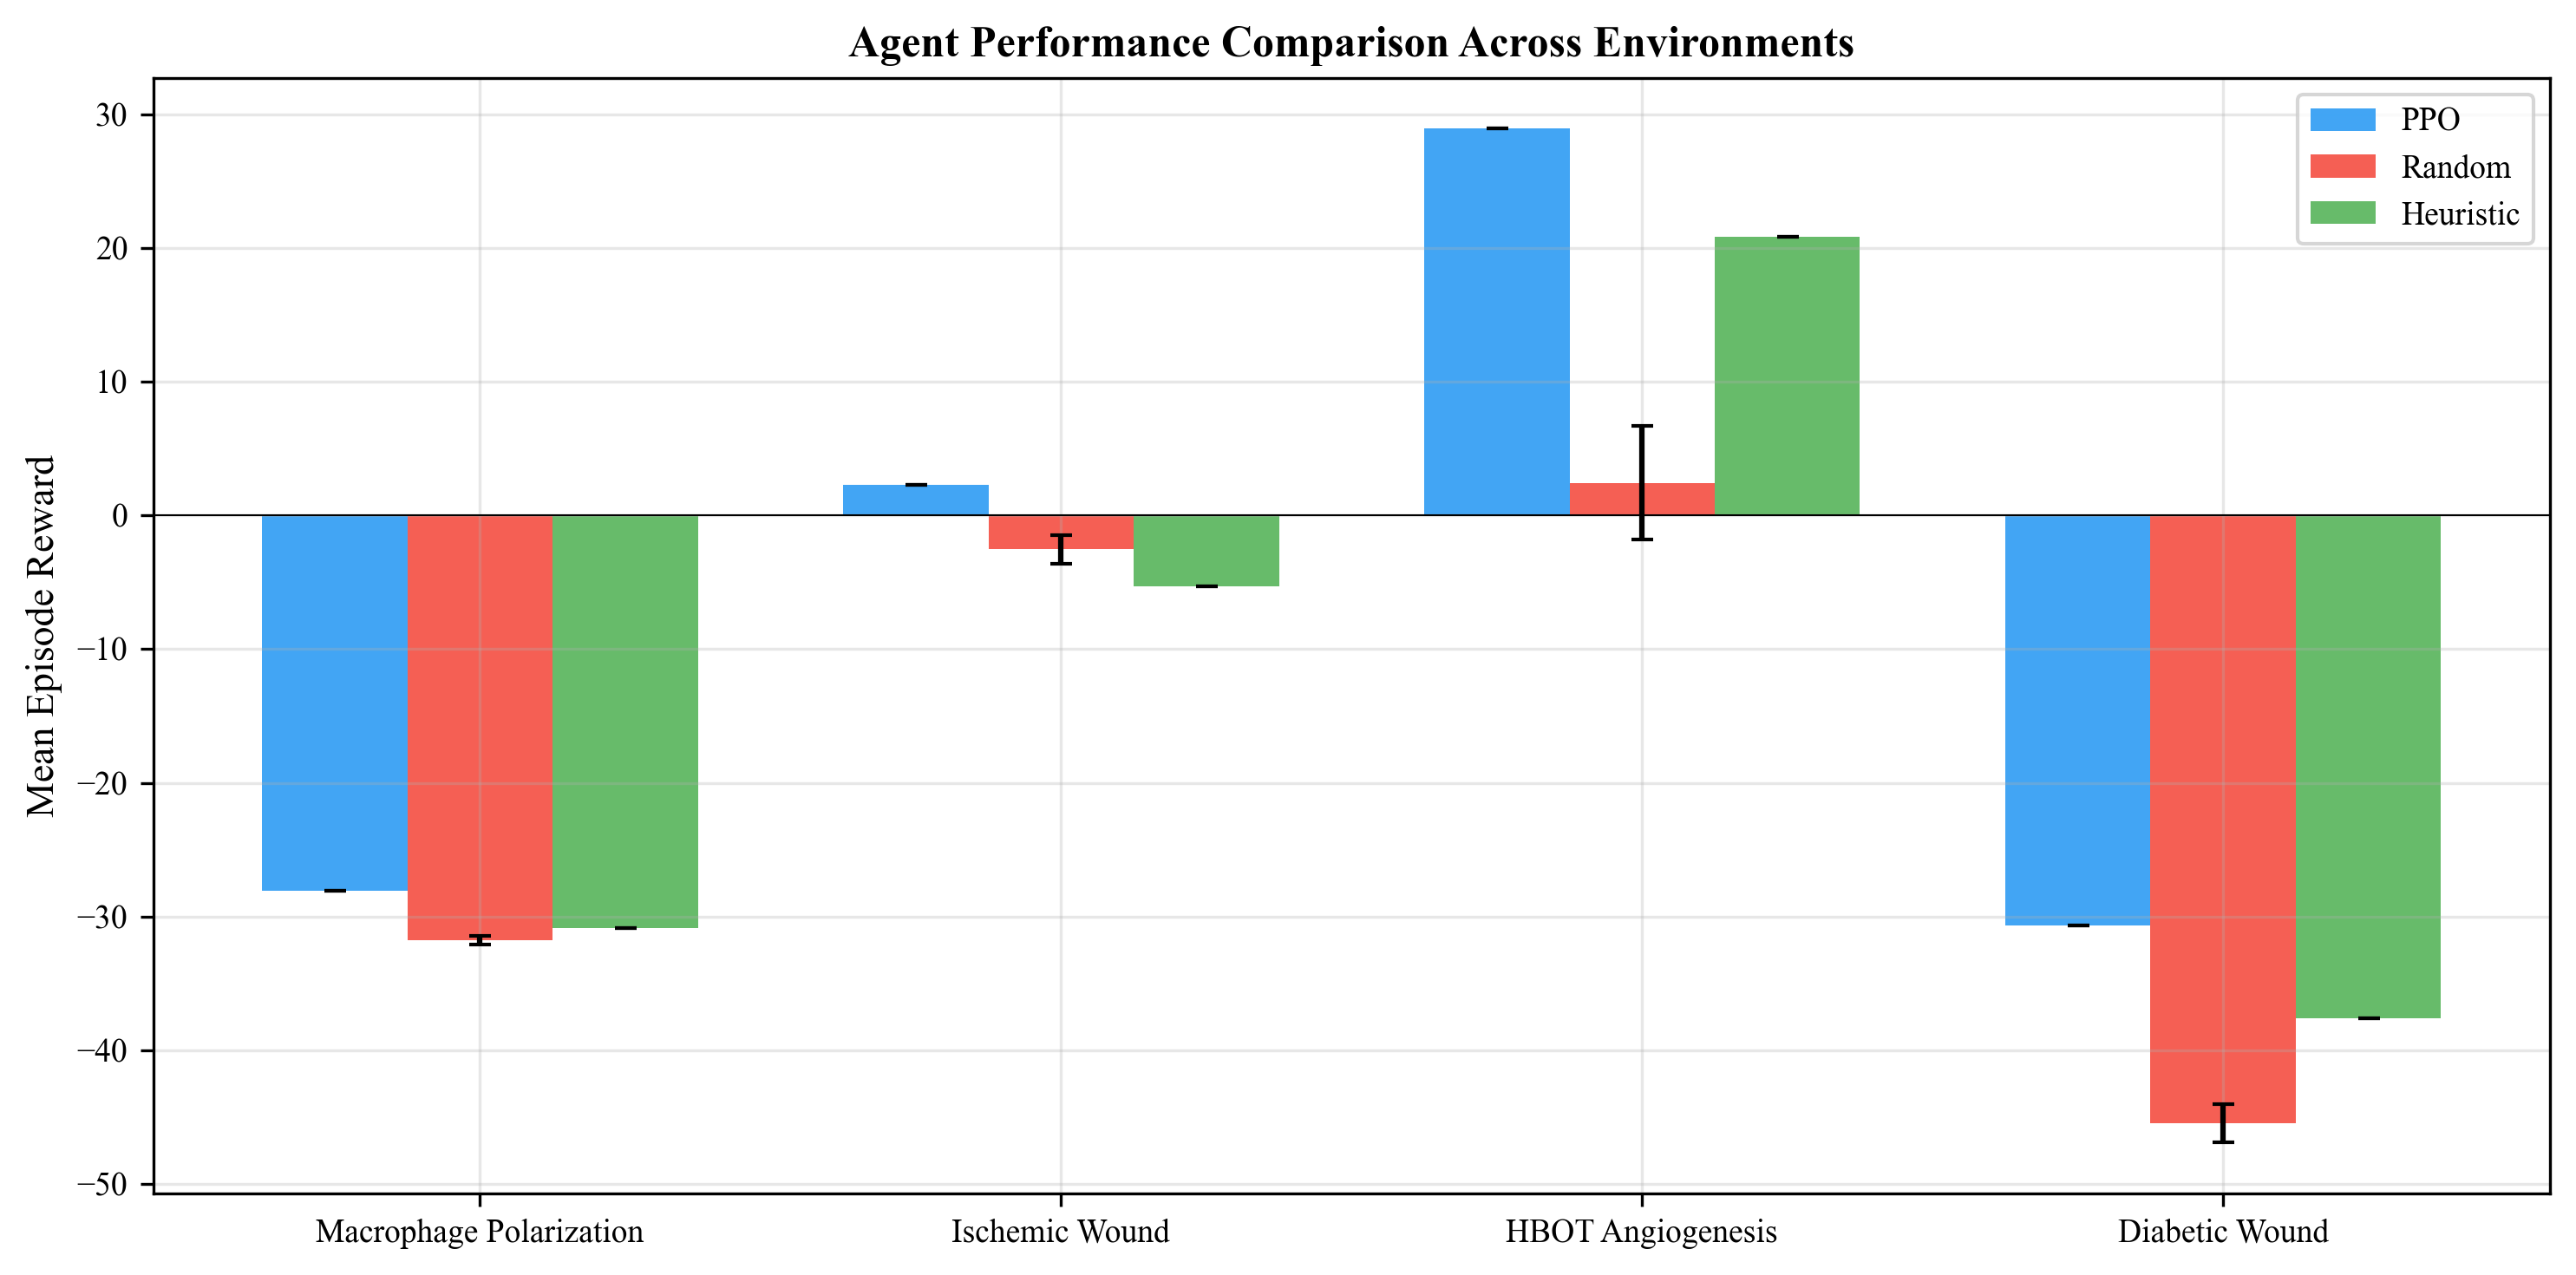
\includegraphics[width=0.9\textwidth]{figures/baseline_comparison.png}
\caption{Mean episode reward comparison across agents and environments. Error bars indicate one standard deviation over 50 evaluation episodes.}
\label{fig:comparison}
\end{figure}

\subsection{Analysis of Learned Policies}

Several patterns emerge from the results:

\paragraph{HBOT: Exploiting the Angiogenesis Paradox.}
The HBOT environment exhibits the largest PPO advantage. The learned policy discovers that moderate, state-dependent oxygen delivery maintains oxygen below the angiogenesis-suppression threshold ($O_{\text{thresh}} = 40$ mmHg) during the critical early vascularization phase, then increases intensity once sufficient capillary density is established. The heuristic baseline, with its fixed moderate protocol, cannot adapt to the wound's evolving state.

\paragraph{Diabetic: Joint Wound--Glycemic Optimization.}
PPO achieves a 33\% improvement over random on the diabetic environment, which requires simultaneous wound treatment and insulin management. The learned policy coordinates insulin dosing with polarization treatment, recognizing that glucose control is a prerequisite for effective macrophage polarization, a coupling not captured by the independent sliding-scale heuristic.

\paragraph{Ischemic: Learned Revascularization Timing.}
The ischemic environment shows the most dramatic qualitative difference: PPO achieves positive cumulative reward ($+2.31$) while both baselines produce negative returns. The learned policy modulates revascularization intensity based on the current oxygen deficit and VEGF concentration, rather than applying constant maximum treatment.

\paragraph{Macrophage: Adaptive Polarization.}
Even on the simplest environment, PPO learns a time-varying polarization strategy that outperforms the constant $u = 0.5$ heuristic by 9\%, demonstrating that dynamic treatment adaptation provides benefit even with a single action dimension.

\section{Discussion}

\subsection{Environment Complexity Spectrum}

WoundSim environments span a deliberate complexity gradient: 4 state variables and 2 actions (HBOT) to 7 state variables and 3 actions (Diabetic). This supports progressive research: algorithms validated on simpler environments can be extended to more complex ones within the same framework.

\subsection{Biological Fidelity and Limitations}

All ODE parameters carry explicit source annotations to their origin publications. However, several simplifications merit discussion:

\begin{itemize}
    \item \textbf{Spatial averaging}: All models are ODE (well-mixed) approximations of inherently spatial processes. The original Xue--Friedman model \citep{xue2009} includes spatial PDE terms that we omit for RL tractability.
    \item \textbf{Parameter normalization}: Cell densities are normalized to $[0, 1]$ carrying capacity to improve RL training stability. Rates are adjusted accordingly.
    \item \textbf{Deterministic dynamics}: Real wound healing involves stochastic cellular processes. WoundSim environments are deterministic given fixed initial conditions (except for the optional noise in the macrophage hard tier).
    \item \textbf{Glucose model simplicity}: The diabetic environment uses a reduced glucose--insulin model. Full models (e.g., Bergman minimal model) would add physiological fidelity at the cost of additional complexity.
\end{itemize}

\subsection{Comparison to Prior Work}

\citet{lu2024} report PPO results on a single macrophage polarization environment. Our Macrophage environment uses the same underlying \citet{zlobina2022} ODE system but extends the benchmark in three directions: (1)~additional wound types requiring qualitatively different treatment strategies, (2)~clinical heuristic baselines providing stronger comparison than random or constant policies alone, and (3)~a standardized, pip-installable interface enabling direct reproduction.

\subsection{Potential Clinical Applications}

While WoundSim is a research tool, the environments model clinically relevant treatment decisions: HBOT session planning, growth factor dosing, and insulin management for diabetic wounds. Policies trained on these environments could inform clinical decision support systems, particularly for identifying counter-intuitive treatment strategies (e.g., the HBOT moderation policy) that may not emerge from standard clinical guidelines.

\section{Architecture}

\begin{figure}[h]
\centering
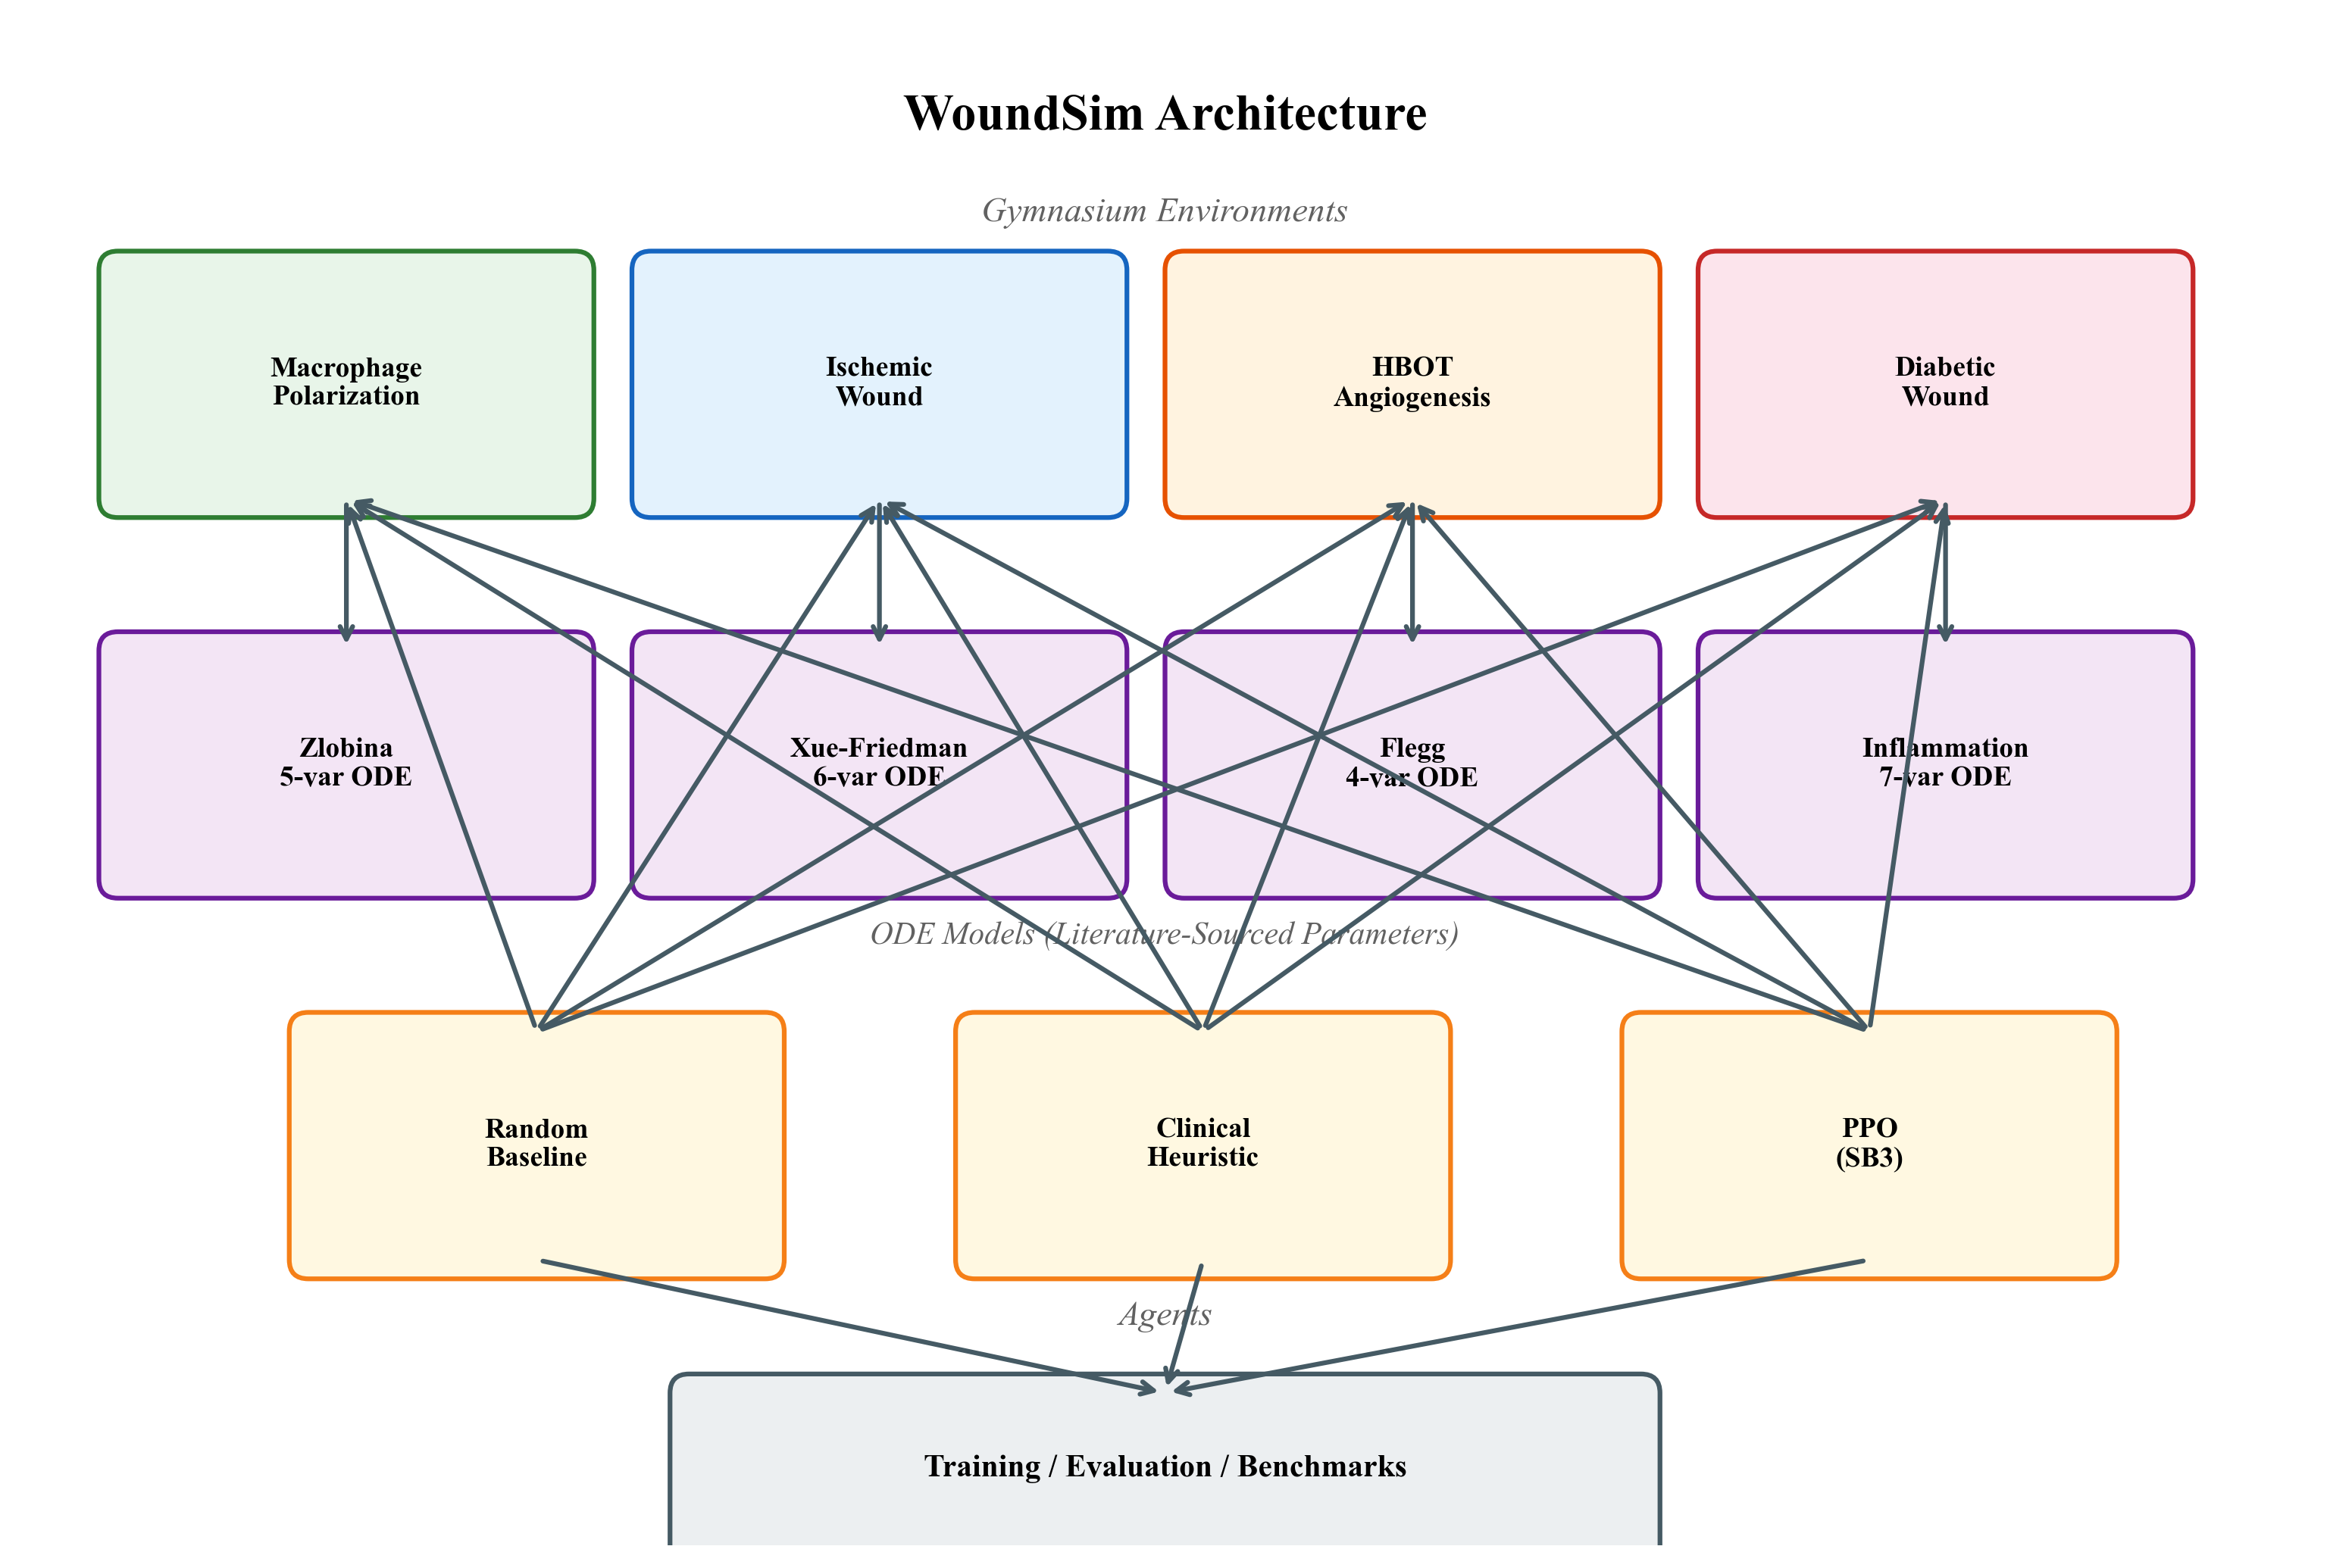
\includegraphics[width=0.85\textwidth]{figures/architecture.png}
\caption{WoundSim architecture. ODE models (bottom) are wrapped by Gymnasium environments (middle) exposing a standard \texttt{reset}/\texttt{step} API. Training scripts and heuristic baselines (top) interact through the Gymnasium interface.}
\label{fig:architecture}
\end{figure}

The package is organized into three layers: (1)~\texttt{models/} containing pure ODE implementations with no RL dependencies, (2)~\texttt{envs/} wrapping each model as a Gymnasium environment with normalization, reward shaping, and difficulty configuration, and (3)~\texttt{agents/} and \texttt{training/} providing heuristic baselines and PPO training infrastructure. This separation enables model reuse outside the RL context (e.g., for optimal control research).

\section{Conclusion}

We introduced WoundSim, a suite of four Gymnasium-compatible RL environments grounded in published ODE models of wound healing. The package provides validated biological dynamics across four wound types, clinical heuristic baselines, configurable difficulty tiers, and full Stable-Baselines3 compatibility. PPO experiments demonstrate meaningful policy differentiation: learned treatment strategies outperform both random and clinical heuristic baselines in every environment, with the HBOT environment exhibiting an $11.9\times$ improvement over random policy. WoundSim enables reproducible, biologically grounded RL research on wound healing treatment optimization.

The package is available at \url{https://pypi.org/project/woundsim/} and \url{https://github.com/HassDhia/woundsim}.

\section*{Acknowledgments}

We thank the authors of the original wound healing models (Zlobina \& Gomez, Xue, Friedman \& Sen, Flegg, Byrne \& McElwain, and Waugh \& Sherratt) whose rigorous mathematical modeling made this work possible.

\bibliographystyle{plainnat}
\bibliography{references}

\appendix

\section{Model Parameters}
\label{app:params}

\begin{table}[h]
\centering
\caption{Macrophage polarization model parameters (Zlobina et al., 2022).}
\begin{tabular}{@{}llrl@{}}
\toprule
Symbol & Description & Value & Source \\
\midrule
$\gamma_a$ & Debris clearance rate & 0.003 day$^{-1}$ & zlobina2022 \\
$s_m$ & M1 recruitment rate & 0.8 day$^{-1}$ & zlobina2022 \\
$K_a$ & Debris half-saturation & 0.3 & zlobina2022 \\
$\mu_m$ & Macrophage death rate & 0.1 day$^{-1}$ & zlobina2022 \\
$\delta$ & Polarization rate & 0.3 day$^{-1}$ & zlobina2022 \\
$s_{m2}$ & M2 recruitment from tissue & 0.4 day$^{-1}$ & zlobina2022 \\
$K_c$ & Tissue half-saturation & 0.3 & zlobina2022 \\
$s_c$ & Granulation production & 0.06 day$^{-1}$ & zlobina2022 \\
$K_{m2}$ & M2 half-saturation & 0.5 & zlobina2022 \\
$\mu_c$ & Tissue remodeling rate & 0.08 day$^{-1}$ & zlobina2022 \\
$s_n$ & Permanent tissue formation & 0.015 day$^{-1}$ & zlobina2022 \\
$\mu_n$ & Tissue turnover & 0.02 day$^{-1}$ & zlobina2022 \\
\bottomrule
\end{tabular}
\end{table}

\begin{table}[h]
\centering
\caption{Ischemic wound model parameters (Xue, Friedman \& Sen, 2009).}
\begin{tabular}{@{}llrl@{}}
\toprule
Symbol & Description & Value & Source \\
\midrule
$k_{\text{close}}$ & Wound closure rate & 0.01 day$^{-1}$ & xue2009 \\
$K_F$ & Fibroblast half-saturation & 0.3 & xue2009 \\
$k_{\text{open}}$ & Ischemic opening rate & 0.015 day$^{-1}$ & xue2009 \\
$O_{\text{crit}}$ & Critical oxygen & 40 mmHg & xue2009 \\
$\alpha_O$ & Oxygen supply rate & 0.3 day$^{-1}$ & xue2009 \\
$O_{\text{blood}}$ & Arterial oxygen & 80 mmHg & xue2009 \\
$s_M$ & Macrophage recruitment & 0.5 day$^{-1}$ & xue2009 \\
$s_F$ & Fibroblast recruitment & 0.15 day$^{-1}$ & xue2009 \\
$s_E$ & ECM production & 0.05 day$^{-1}$ & xue2009 \\
\bottomrule
\end{tabular}
\end{table}

\begin{table}[h]
\centering
\caption{HBOT angiogenesis model parameters (Flegg et al., 2009, 2015).}
\begin{tabular}{@{}llrl@{}}
\toprule
Symbol & Description & Value & Source \\
\midrule
$s_b$ & Tip sprouting rate & 0.4 day$^{-1}$ & flegg2009 \\
$O_{\text{thresh}}$ & Angiogenesis threshold & 40 mmHg & flegg2009 \\
$K_b$ & Tip half-saturation & 10 mmHg & flegg2009 \\
$d_b$ & Tip death rate & 0.15 day$^{-1}$ & flegg2009 \\
$\chi$ & Chemotactic sensitivity & 0.05 & flegg2009 \\
$O_{\text{ref}}$ & Reference oxygen level & 20 mmHg & flegg2009 \\
$\alpha_n$ & Tip-to-sprout conversion & 0.12 day$^{-1}$ & flegg2009 \\
$P_O$ & Capillary $O_2$ production & 15 mmHg/day & flegg2010 \\
$\lambda_O$ & Oxygen decay rate & 0.3 day$^{-1}$ & flegg2010 \\
$D_{\text{ext}}$ & HBOT delivery coeff. & 50 & flegg2010 \\
$k_{\text{heal}}$ & Healing rate & 0.01 day$^{-1}$ & flegg2009 \\
\bottomrule
\end{tabular}
\end{table}

\begin{table}[h]
\centering
\caption{Diabetic wound model parameters. Macrophage parameters adapted from \citet{zlobina2022}; glucose--insulin dynamics from \citet{waugh2006}; ECM from \citet{xue2009}.}
\begin{tabular}{@{}llrl@{}}
\toprule
Symbol & Description & Value & Source \\
\midrule
$k_w$ & Wound closure rate & 0.004 day$^{-1}$ & waugh2006 \\
$k_d$ & Debris generation rate & 0.05 day$^{-1}$ & zlobina2022 \\
$\gamma_a$ & Debris clearance rate & 0.08 day$^{-1}$ & zlobina2022 (adapted) \\
$s_m$ & M1 recruitment rate & 0.6 day$^{-1}$ & zlobina2022 (adapted) \\
$K_a$ & Debris half-saturation & 0.3 & zlobina2022 \\
$\mu_m$ & Macrophage death rate & 0.1 day$^{-1}$ & zlobina2022 \\
$\delta_{\text{base}}$ & Base polarization rate & 0.25 day$^{-1}$ & zlobina2022 (adapted) \\
$G_{\text{target}}$ & Target glucose & 100 mg/dL & waugh2006 \\
$k_{\text{ins}}$ & Insulin sensitivity & 0.05 & waugh2006 \\
$k_{gc}$ & Glucose clearance rate & 0.01 day$^{-1}$ & waugh2006 \\
$G_{\text{prod}}$ & Hepatic glucose production & 2.0 mg/dL/hr & waugh2006 \\
$G_{\text{imp}}$ & Impairment threshold & 180 mg/dL & waugh2006 \\
$k_{\text{imp}}$ & Impairment steepness & 0.5 & waugh2006 \\
$s_E$ & ECM production rate & 0.04 day$^{-1}$ & xue2009 (adapted) \\
$d_E$ & ECM remodeling rate & 0.05 day$^{-1}$ & xue2009 \\
$g_f$ & Growth factor boost & 0.3 day$^{-1}$ & estimated \\
\bottomrule
\end{tabular}
\end{table}

\end{document}
